\documentclass[aspectratio=1610]{beamer}

\usetheme{KTH}
\usepackage[utf8]{inputenc}
\usepackage{graphics}
\usepackage{graphicx}
\usepackage{booktabs}
\usepackage{amsmath}
\usepackage{mathtools}
\usepackage[makeroom]{cancel}
\usepackage[utf8]{inputenc}
\usepackage{amssymb}
\usepackage{ragged2e}
\usepackage{lipsum}
\usepackage{tikz}
\usepackage{array}
\usepackage{amsmath,amsfonts,amssymb}
\usepackage[export]{adjustbox}

\usefonttheme{serif}


\begin{document}
\begin{frame}[noframenumbering,plain]

  \vspace{0.02\textheight}
  
\begin{columns}[]
\column{37em}
\Large{\centerline{\usebeamercolor[fg]{title}Mästarprov 13: Strömkretsen}}

\vspace{0.1\textheight}

\small{\centerline{Hassan Al Noori}}
\scriptsize{\centerline{\tt hassanan@kth.se}}
\scriptsize{\centerline{}}
\end{columns}
\end{frame}

%------------------------------------------------
\usebackgroundtemplate{\vbox{\null\vspace{3mm}
  \hspace{3mm}\pgfuseimage{kthlogosmall}\par
  \vspace{72mm}\hbox{\hspace{-75mm}\pgfuseimage{kthplatta}}}}

%------------------------------------------------
\begin{frame}
\begin{columns}
\column{37em}
\hspace*{2cm}\includegraphics[width=10cm]{figs/Stromkrets.png}
\end{columns}
\end{frame}
%------------------------------------------------
\begin{frame}
\frametitle{LC-circuit}
\begin{columns}
\column{37em}
\begin{itemize}
    \item What is an LC-circuit?
\end{itemize}
\end{columns}
\end{frame}
%------------------------------------------------
\begin{frame}
\frametitle{RFID}
\begin{columns}
\column{37em}
\hspace*{5cm}\includegraphics[width=5cm]{figs/rfid.png}
\end{columns}
\end{frame}
%------------------------------------------------
\begin{frame}
\frametitle{Electronic article surveillance}
\begin{columns}
\column{37em}
\hspace*{5cm}\includegraphics[width=4cm]{figs/barcode.png}
\end{columns}
\end{frame}
%------------------------------------------------
\begin{frame}
\frametitle{Project requirements}
\begin{columns}
\column{37em}
\begin{itemize}\itemsep1em
  \item<1-> What is the current in the circuit?
  \item<2-> How is the current affected by the voltage?
\end{itemize}
\end{columns}
\end{frame}
%------------------------------------------------
\begin{frame}
\frametitle{Mathematical equations}
\begin{columns}
\column{37em}
\hspace*{2cm}\includegraphics[width=2.7cm]{figs/inductance.png}
\hspace*{2cm}\includegraphics[width=2.7cm]{figs/voltage.png}
\hspace*{2cm}\includegraphics[width=2.7cm]{figs/current.png}
\hspace*{2cm}\includegraphics[width=5.4cm]{figs/initial values.png}
\end{columns}
\end{frame}
%------------------------------------------------
\begin{frame}
\frametitle{Mathematical equations}
\begin{columns}
\column{37em}
\hspace*{2cm}\includegraphics[width=9cm]{figs/2nd ODE.png}
\end{columns}
\end{frame}
%------------------------------------------------
\begin{frame}
\frametitle{Mathematical equations}
\begin{columns}
\column{37em}
\hspace*{2cm}\includegraphics[width=11cm]{figs/2nd ode.png}
\end{columns}
\end{frame}
%------------------------------------------------
\begin{frame}
\frametitle{Numerical Methods - Runge Kutta 4}
\begin{columns}
\column{2em}
  \begin{align*}
  K_{1}&=hf(x_{n},y_{n})\\
  K_{2}&=hf(x_{n}+\frac{h}{2},y_{n}+\frac{k_{1}}{2})\\
  K_{3}&=hf(x_{n}+\frac{h}{2},y_{n}+\frac{k_{2}}{2})\\
  K_{4}&=hf(x_{n}+h,y_{n}+k_{3})\\
  y_{n+1}&=y_{n}+\frac{1}{6}\left(K_{1}+2K_{2}+2K_{3}+K_{4}\right)+O(h^{5})
  \end{align*}
\end{columns}
\end{frame}

%------------------------------------------------
\begin{frame}
  \frametitle{Frame title}
  
      \centerline{\includegraphics[scale=0.5]{figs/240V + E.pdf}}
  \begin{center}
  \end{center}	
  \end{frame}
%------------------------------------------------
\begin{frame}
\frametitle{Numerical Results}
\begin{columns}
%\column{37em}
\includegraphics[scale=0.5]{{figs/240V + E.pdf}}
%\centerline{\vspace*{1cm}\includegraphics[width=11cm]{figs/240V + E.pdf}}
\end{columns}
\end{frame}
%------------------------------------------------
\begin{frame}
\frametitle{Numerical Results}
\begin{columns}
\column{37em}
\centerline{\vspace*{2cm}\includegraphics[width=8cm]{figs/1200V + E.jpg}}
\end{columns}
\end{frame}
%------------------------------------------------
\begin{frame}
\frametitle{Numerical Results}
\begin{columns}
\column{37em}
\centerline{\vspace*{2cm}\includegraphics[width=8cm]{figs/2400V + E.jpg}}
\end{columns}
\end{frame}
%------------------------------------------------
\
\end{document}
